%%%%%%%%%%%%%%%%%%%%%%%%%%%%%%%%%%%%%%%%%%%%%%%%%%%%%%%%%%%%%%%%%%%%%%%%%%%%%%%
%%%%%%%%%%%%%%%%%%%%%%%%%%%%%%%%%%%%%%%%%%%%%%%%%%%%%%%%%%%%%%%%%%%%%%%%%%%%%%%
%%%%%%%%%%%%%%%%%%%%%%%%%%%%%%%%%%%%%%%%%%%%%%%%%%%%%%%%%%%%%%%%%%%%%%%%%%%%%%%

\section{Aplikace \texttt{the\_next\_word\_prediction}}%
\index{aplikace!\texttt{the\_next\_word\_prediction}}

Aplikace, podobně jako asynchronní úlohy\index{úloha!asynchronní} v rámci zpracování textu%
\index{processing}
korpusu\index{korpus} a~$n$-grammingu\index{$n$-gram}, byla vyvinuta v jazyce
\textsf{R}\index{\textsf{R}} prostřednictvím
\textsf{R}-kového balíčku \texttt{Shiny}\index{\texttt{Shiny}}.

Smyslem aplikace je nabídnout platformu pro predikci slova\index{$n$-té slovo!predikce}, které s největší
pravděpodobností\index{pravděpodobnost} následuje zadané anglické $(n - 1)$-členné sousloví%
\index{$(n - 1)$-členná fráze}, kde
$n > 1$.


\subsection{Princip aplikace}
\label{subsec:princip_aplikace}

Zadá-li uživatel do aplikace $(n - 1)$-členné anglické sousloví%
\index{$(n - 1)$-členná fráze}, kde $n > 1$,
s cílem odhadnout slovo, které by mělo dané $(n - 1)$-členné sousloví%
\index{$(n - 1)$-členná fráze}
s největší pravděpodobností\index{pravděpodobnost} následovat, aplikace najde největší
takové $n_{0}$, aby $0 \leq n_{0} \leq n - 1$ a zároveň aby v množině
všech $\{2, 3, 4, 5\}$-gramů\index{$n$-gram} existoval alespoň jeden
takový $(n_{0} + 1)$-gram\index{$n$-gram},
že posledních $n_{0}$ slov uživatelem zadaného sousloví odpovídá postupně
prvnímu, druhému, \ldots, $n_{0}$-tému slovu tohoto $(n_{0} + 1)$-gramu%
\index{$n$-gram}.
Ze všech takto vyhovujících $(n_{0} + 1)$-gramů je pak vybrán ten, který má
největší relativní četnost (v korpusu\index{korpus}, resp. ve frekvenční tabulce%
\index{$n$-gram!tabulka četností}
$(n_{0} + 1)$-gramů) a jeho $(n_{0} + 1)$-té slovo je vráceno uživateli
jako to, které nejpravděpodobněji následuje jeho zadanou
$(n - 1)$-člennou frázi\index{$(n - 1)$-členná fráze}.

Jinými slovy a formálněji, uvažujme, že uživatel zadá do aplikace na
vstupu \mbox{$(n -1)$-člennou} frázi%
\index{$(n - 1)$-členná fráze} ve tvaru $w_{1}w_{2} \ldots w_{n - 1}$,
kde $w_{j}$ je $j$-té slovo\index{slova} dané fráze postupně pro všechna
$j \in \{ 1, 2, \ldots, n - 1 \}$, s cílem zjistit, jaké slovo $w_{n}$%
\index{$n$-té slovo}
bude nejpravděpodobněji\index{pravděpodobnost} následovat po zadaných $n - 1$ slovech ve frázi%
\index{$(n - 1)$-členná fráze}.
Buď $\mathcal{G}_{n} = \{v_{1}v_{2} \ldots v_{n} \mid n\}$ množina všech
známých $n$-gramů\index{$n$-gram}, postupně pro všechna $n \in \{2, 3, 4, 5\}$.
Hledáme $n_{0}$ takové, aby

\begin{equation*}
  n_{0} = \argmax_{i \in \{ 0, 1, \ldots, n - 1 \}} \{i : 
  (\exists v_{1}v_{2} \ldots v_{i + 1} \in \mathcal{G}_{i + 1})
  (\forall j \in \{1, 2, \ldots, i\})(v_{j} = w_{n - i + j - 1}) \}.
\end{equation*}

Je-li $n_{0} = 0$, aplikace vrátí nejčastější unigram\index{$n$-gram!unigram} (slovo \textit{the})%
\index{člen \textit{the}}.
Je-li však $n_{0} > 0$, pak označme $\mathcal{G}_{n_{0} + 1}^{*}$ množinu
všech $(n_{0} + 1)$-gramů\index{$n$-gram}, které jsou tvaru $v_{1}v_{2} \ldots v_{n_{0} + 1} =
w_{n - n_{0}}w_{n - n_{0} + 1} \ldots w_{n - 1}$. Potom slovo, které
nejpravděpodobněji následuje uživatelovu frázi\index{$(n - 1)$-členná fráze}
$w_{1}w_{2} \ldots w_{n - 1}$, je $w_{n}^{*}$ takové, že\index{pravděpodobnost!odhad}

\vspace{-1.0cm}
\begin{align*}
  \phantom{n_{0}} &\phantom{= \argmax_{i \in \{ 0, 1, \ldots, n - 1 \}} \{i : 
  (\exists v_{1}v_{2} \ldots v_{i + 1} \in \mathcal{G}_{i + 1})
  (\forall j \in \{1, 2, \ldots, i\})(v_{j} = w_{n - i + j - 1}) \}.} \\
  w_{n}^{*} &= \argmax_{v_{1}v_{2} \ldots w_{n} \in \mathcal{G}_{n_{0}
  + 1}^{*}} \{
  \hat{P}(w_{n}^{*} = v_{n_{0} + 1} \mid v_{1}v_{2} \ldots v_{n_{0} + 1} \in 
  \mathcal{G}_{n_{0} + 1}^{*} ) \}.
\end{align*}

Jde o MAP (\underline{m}aximum \underline{a}posteriori \underline{p}robability)
princip\index{algoritmus!maximum aposteriori}, kdy je jako
nejpravděpodobnější $n$-té slovo\index{$n$-té slovo} následující uživatelovu
$(n - 1)$-člennou frázi\index{$(n - 1)$-členná fráze} vybráno poslední slovo
takového $(n_{0} + 1)$-gramu\index{$n$-gram},
který má prvních $n_{0}$ slov totožných s posledními $n_{0}$ slovy uživatelovy
fráze a zároveň je mezi takovými $(n_{0} + 1)$-gramy nejčastěji zastoupen.
Je-li více takových nejčastěji zastoupených $(n_{0} + 1)$-gramů, je jako
$n$-té slovo následující uživatelovu frázi vybráno to, které je první
v abecedě (anebo je vybráno poslední slovo náhodného z těchto $n$-gramů).
Někdy se též popsanému přístupu říká back-off model%
\index{$n$-té slovo!predikce!back-off}, neboť algoritmus
v podstatě nejdříve vyhledává shodu se zadanou frází mezi $n$-gramy\index{$n$-gram};
pokud
ji nenajde, pokračuje mezi $(n - 1)$-gramy, opět pokud ji nenalezne,
přistoupí k $(n - 2)$ gramům, a tak dále, až nakonec prohledává $1$-gramy
(unigramy)\index{$n$-gram!unigram}. Když nenalezne shodu mezi žádným unigramem a posledním slovem
uživatelovy fráze, vrací obvykle nejčastější unigram (v angličtině člen
\textit{the}\index{člen \textit{the}}).

Kromě MAP principu\index{algoritmus!maximum aposteriori}
existují i další, sofistikovanější přístupy, jak vybrat
nejpravděpodobnější $n$-té slovo doplňující uživatelovu $(n - 1)$-člennou
frázi\index{$(n - 1)$-členná fráze}. Někdy se případy chybějících frází ošetřují obyčejným
Laplaceovým
"add-one" vyhlazováním~\cite{Chen1996}\index{vyhlazování!Laplaceovo (add-one)}, kdy je každému $n$-gramu%
\index{$n$-gram}
(i chybějícímu, poprvé se objevivšímu až při uživatelově zadání) uměle
zvýšena absolutní četnost ve frekvenčních tabulkách $n$-gramů\index{$n$-gram!tabulka četností} o $1$.
Obecně se tento přístup dnes již nedoporučuje. Známé je také
např. Kneser-Neyovo vyhlazování~\cite{Jurafsky2009}\index{vyhlazování!Kneser-Neyovo},
které pro danou $(n - 1)$-člennou frázi\index{$(n - 1)$-členná fráze},
jež zadává uživatel, prohledává
i po nalezení dobré shody mezi posledními $n_{0}$ slovy uživatelovy fráze
a~některým $(n_{0} + 1)$-gramem\index{$n$-gram} ještě všechny $(n_{0} + 1 - j)$-gramy pro
$\forall j \in \{1, 2, \ldots, n_{0}\}$ a zkoumá četnosti dalších shodujících
se $(n_{0} + 1 - j)$-gramů s posledními $(n_{0} - j)$ slovy uživatelovy
fráze -- pokud by některá četnost některé $(n_{0} + 1 - j)$-gramu byla
výrazně vyšší než byla četnost nejčastějšího $(n_{0} + 1)$-gramu,
jako uživatelem hledané slovo je (poněkud paradoxně) vráceno poslední
slovo tohoto (i podstatně kratšího) $(n_{0} + 1 - j)$-gramu. Kneser-Neyovo
vyhlazování\index{vyhlazování!Kneser-Neyovo} totiž řeší
i kontextové zařazení některých frází.


\subsection{Komponenty aplikace}

Aplikace\index{aplikace!\texttt{the\_next\_word\_prediction}} se skládá z následujících částí:

\begin{itemize}
  \item \texttt{ui.R}
  \item \texttt{server.R}
  \item slovníky $n$-gramů\index{$n$-gram}, tedy \texttt{my\_$i$\_word\_vocabulary}
        pro $i \in \{1, 2, 3\}$
  \item složka \texttt{www}:
  \begin{itemize}
    \item \texttt{style.css}\index{CSS}
  \end{itemize}
\end{itemize}


Uživatelský layout aplikace je relativně jednoduchý a intuitivní, viz
obrázek~\ref{layout_fig}.

\begin{figure}[h]
  \centering
  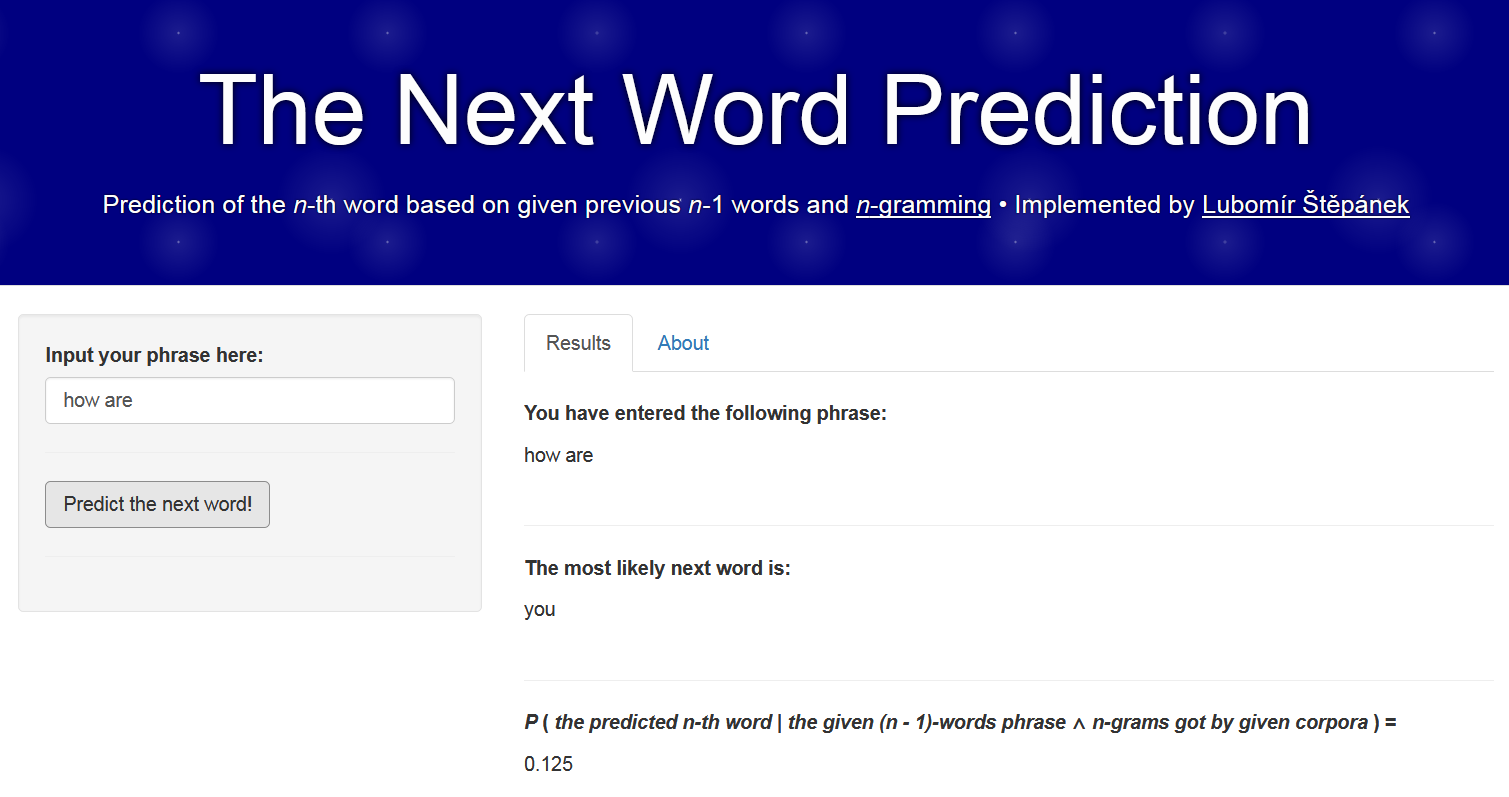
\includegraphics[width = \textwidth]{layout.png}
  \caption{Uživatelský interface domovské stránky aplikace}\label{layout_fig}
\end{figure}

Online lze aplikaci používat snadno na adrese\index{\texttt{Shiny}}

\begin{center}
  \href{http://shiny.statest.cz:3838/the\_next\_word\_prediction/}{%
    http://shiny.statest.cz:3838/the\_next\_word\_prediction/
  }.
\end{center}

Na první záložce \textit{Results} lze vložit vstupní frázi o délce 1-3 slov.
Po kliknutí na tlačítko \textit{Predict the next word!}\index{$n$-té slovo!predikce} se v pravém
panelu zobrazí slovo, které by mělo pravděpodobně jazykově následovat
po vložené $(n - 1)$-členné frázi\index{$(n - 1)$-členná fráze}.

Na druhé záložce \textit{About} je zmíněno pár slov o účelu a principu aplikace.

Popišme nyní detailněji jednotlivé části aplikace.

\begin{labeling}{a b c d e f g h i j k}\index{\texttt{Shiny}}

  \item [\texttt{ui.R}] Viz též~\ref{ui}. Název vyplývá ze zkratky
  \textit{\underline{u}ser \underline{i}nterface}. Definuje veškeré grafické
  a ovládací prvky aplikace, které lze napsat pomocí jazyka HTML\index{HTML}
  (\underline{H}yper\underline{T}ext \underline{M}arkup \underline{L}anguage).
  I přesto je však psána pomocí příkazů jazyka \textsf{R}\index{\textsf{R}}; balíček
  \texttt{Shiny}\index{\texttt{Shiny}} totiž definuje placeholderové funkce (aliasy), které mají na
  vstupu kód srozumitelný prostředí \textsf{R}\index{\textsf{R}}, ale na výstupu vrací čisté
  HTML\index{HTML}. Některé grafické prvky však byly napsány přímo pomocí syntaxe HTML%
  \index{HTML}
  -- balíček \texttt{Shiny}\index{\texttt{Shiny}} této syntaxi rozumí a v případě, že má uživatel
  znalost i značkovacího jazyka HTML\index{HTML}, je pak práce snazší přímo pomocí HTML,
  nikoliv \textsf{R}-kových aliasů či wrapperů.
  
  \item [\texttt{server.R}] Viz též~\ref{server}. Jádro celé aplikace,
  obsahuje workhorse funkce, především implementaci backoff modelu výběru tak,
  jak je popsán ve stati~\ref{subsec:princip_aplikace}.
  
  \item [slovníky $n$-gramů] Viz též tabulka~\ref{trigramy}\index{$n$-gram!trigram}
  a komponenta~\ref{bigram}\index{$n$-gram!bigram}. Slovníky tvoří základ pro back-off vyhledávání%
  \index{$n$-té slovo!predikce!back-off}
  nejpravděpodobnějšího $n$-tého slova následujícího $(n - 1)$-člennou frázi%
  \index{$(n - 1)$-členná fráze}.
 
  \item [\texttt{style.css}] Viz též~\ref{style}. Kaskádové styly\index{CSS}, které
  definují rozměry, barvy a další parametry některých prvků aplikace, především
  headeru.

  
\end{labeling}


\newpage


%%%%%%%%%%%%%%%%%%%%%%%%%%%%%%%%%%%%%%%%%%%%%%%%%%%%%%%%%%%%%%%%%%%%%%%%%%%%%%%
%%%%%%%%%%%%%%%%%%%%%%%%%%%%%%%%%%%%%%%%%%%%%%%%%%%%%%%%%%%%%%%%%%%%%%%%%%%%%%%
%%%%%%%%%%%%%%%%%%%%%%%%%%%%%%%%%%%%%%%%%%%%%%%%%%%%%%%%%%%%%%%%%%%%%%%%%%%%%%%





